\documentclass[11pt]{article}
\usepackage[margin=1in]{geometry}
\usepackage{amsmath,amssymb,amsthm}
\usepackage{graphicx}
\usepackage{booktabs}
\usepackage[colorlinks=true,linkcolor=blue,citecolor=blue,urlcolor=blue]{hyperref}
\usepackage{xcolor}

\newtheorem{theorem}{Theorem}
\newtheorem{proposition}{Proposition}
\newtheorem{conjecture}{Conjecture}
\newtheorem{remark}{Remark}

\newcommand{\sgn}{\operatorname{sgn}}

\title{The Island Has Edges:\\ Exact Boundary Laws for Unitary Deformations\\ of the Veneziano Amplitude}
\author{Andrei Pluzhnik\thanks{ORCID 0009-0005-5660-2603. Code and data are
released as an ancillary package (repository and DOI to accompany this
preprint).}}
\date{August 2026}

\begin{document}
\maketitle

\begin{abstract}
The three-parameter family $(q,r,w)$ of Veneziano deformations constructed by
Cheung, Hillman and Remmen from level truncation and crossing constraints is
restricted by partial-wave positivity to an ``island'' in parameter space,
previously mapped numerically at level depth $n\le 10$. We derive exact
closed-form sign laws for the near-leading Regge partial waves of this family
at $q=1$ and obtain: (i) nothing survives left of the line
$r=-(1+\mu_0)/2$ --- an exclusion valid at every level and in every spacetime
dimension $D>3$ (for $\mu_0\le 0$ the allowed region extends up to this line
in our scans; for $\mu_0>0$ threshold constraints cut strictly inside it);
(ii) the erosion of finite-depth islands is explained cell by cell by a
single linear-in-$n$ law, which also removes $176$ false-positive points from a
fine-grained depth-$20$ scan; (iii) the remaining boundary is cut by an
explicit finite set of low-level algebraic curves whose $D$-dependence is a
$1/(D-1)$ tightening, explaining analytically why the island shrinks with
dimension while its left edge stays pinned; and (iv) the resulting analytic
description reproduces $11{,}994$ exact-rational-arithmetic verdicts across
seven mass shifts with zero mismatches. Beyond the edge, every odd
near-leading trajectory eventually turns negative at a threshold our closed
forms predict exactly, while even trajectories remain positive. For $q>1$ we
measure the exact depth at which unitarity excludes the deformation,
$n_{\rm crit}\simeq 1.1\,(q-1)^{-1/2}$, and derive the $-1/2$ exponent from
the quadratic growth of the relative $q$-correction. On the $w=0$ slice our
edge law reproduces the asymptotic contour result of Mansfield and Spradlin;
to our knowledge --- based on a survey of the works citing CHR indexed in
INSPIRE --- the $w\neq 0$ region has not been treated analytically before.
\end{abstract}

\section{Introduction}

The modern S-matrix bootstrap asks which scattering amplitudes are consistent
with unitarity, crossing, and assumed high-energy behavior --- and, in
particular, how special string amplitudes are within that space. Cheung,
Hillman and Remmen (CHR) \cite{CHR2024} showed that elevating the Veneziano
amplitude's \emph{level truncation} property to an axiom, together with
crossing at truncation points, forces a three-parameter family of dual
resonant amplitudes labeled $(q,r,w)$, with spectrum $\mu(n)=[n]_q$; the
Veneziano amplitude sits at $(1,0,0)$. Imposing partial-wave positivity, CHR
mapped numerically (levels $n\le 10$, $D=4$) a broad allowed region --- an
island --- in the $(r,w)$ plane.

Two natural questions were left open. First, what happens to the island as the
positivity depth $n$ grows --- does it erode away, or stabilize, and what is
its true boundary? Second, positivity was imposed numerically; is the boundary
itself computable in closed form? This paper answers both for $q=1$ (with a
quantitative excursion into $q>1$), using exact rational arithmetic throughout
and a derivation strategy simple enough to state in one line: \emph{track the
top coefficients of the level-$n$ residue polynomial through the partial-wave
projection}.

Our results turn the island from a numerical observation into an analytically
described object, with every claim below either derived in closed form,
verified against exact scans, or explicitly labeled as a conjecture.

\section{Setup}

At $q=1$ the level-$n$ residue of the CHR amplitude (their Eq.~(16)) reduces to
\begin{equation}
R(n,t)\;=\;\frac{(2+r+t)_{n-1}\,\bigl(1+r+t+w\bigr)\bigl(1+n+r+w\bigr)}
{(2+r)_n\,(1+r+w)},
\label{eq:residue}
\end{equation}
a degree-$n$ polynomial in $t$ with roots $t=-(2+r+k)$, $k=0,\dots,n-2$, and
$t=-(1+r+w)$. With external masses $\mu_0$ (spectrum $\mu(n)=n+\mu_0$) the
scattering-angle substitution at level $n$ is
$t = \alpha(x-1) - \mu_0$ with $\alpha=(n-3\mu_0)/2$, $x=\cos\theta$. In $D$
spacetime dimensions the partial-wave coefficients $a_{n,\ell}$ are the
Gegenbauer coefficients ($\alpha_G=\tfrac{D-3}{2}$; Legendre for $D=4$) of
$R$ restricted to level $n$. Unitarity requires $a_{n,\ell}\ge 0$ for all
above-threshold levels ($\mu(n)\ge 4\mu_0$, per CHR).

All numerics below use exact rational arithmetic (Python \texttt{Fraction});
the evaluator was validated by two independent routes (the CHR closed form
(A6) versus a first-principles residue-plus-projection computation), which
agree at every tested $(n,\ell,r,w,\mu_0)$ up to a positive $\ell$-dependent
normalization. The \emph{domain} for every sign statement below is
$2+r>0$ and $1+r+w>0$; outside it the positive prefactor in
Eq.~\eqref{eq:residue} flips sign, and the corresponding full sign laws were
checked separately.

\section{The edge theorem}

\begin{theorem}[Left edge]\label{thm:edge}
For $q=1$, $D>3$, $n>3\mu_0$, and $(r,w)$ in the domain,
\begin{equation}
\sgn a_{n,n-1} \;=\; \sgn\!\Bigl[\,n\Bigl(r+\tfrac{1+\mu_0}{2}\Bigr)+w\,\Bigr].
\label{eq:edgelaw}
\end{equation}
\end{theorem}

\begin{proof}[Proof sketch]
Write the monic part of Eq.~\eqref{eq:residue} as
$p(t)=t^n+A\,t^{n-1}+\dots$ with $A=(n-1)(2+r)+\binom{n-1}{2}+(1+r+w)$.
Substituting $t=\alpha x+\beta$ ($\beta=-\alpha-\mu_0$), the coefficient of
$x^{n-1}$ is $\alpha^{n-1}(A+n\beta)$, and
$A+n\beta=n\bigl(r+\tfrac{1+\mu_0}{2}\bigr)+w$.
By parity and degree, $x^{n}$ projects only onto $C^{(\alpha_G)}_{n},
C^{(\alpha_G)}_{n-2},\dots$ and monomials below $x^{n-1}$ of the correct
parity have degree $<n-1$; hence only the $x^{n-1}$ monomial feeds
$C^{(\alpha_G)}_{n-1}$, with a positive projection constant for every $D>3$.
The prefactor in Eq.~\eqref{eq:residue} is positive in the domain, and
$\alpha>0$ above threshold. (At $n=3\mu_0$ exactly, $\alpha=0$ and
$a_{n,n-1}$ vanishes identically.)
\end{proof}

\noindent
\textbf{Consequences.} Nothing with $r<-(1+\mu_0)/2$ and $w>0$ survives:
positivity fails at depth $n>w/|r+\tfrac{1+\mu_0}{2}|$. The edge is
\emph{dimension-universal}: the $x^{n-1}$ coefficient carries no
$D$-dependence. Finite-depth scans overstate the island in a sliver next to
the edge, with erosion depth inversely proportional to the distance.

\textbf{Verification.} Eight ``razor'' predictions of exact zeros were
confirmed in exact arithmetic, including at points never scanned before
(e.g.\ $(r,w)=(-13/25,1/2)$: predicted zero at $n=25$; measured
$a_{24,23}>0$, $a_{25,24}=0$, $a_{26,25}<0$), at $\mu_0=\pm 3/5$, and at
$D=6,10$. Sixty random $(n,r,w)$ draws confirm the full sign law including
prefactor flips outside the domain. An independent adversarial review
re-derived every step and its six-attack falsification script (published with
the code) found no counterexample.

\textbf{The nine casualties.} In depth-graded scans at $\mu_0=0$, exactly nine
cells vanish between $n\le 10$ and $n\le 20$, all at $r=-3/5$: the law
predicts death at $n=10w+1$, matching the measured first-negative list cell by
cell ($w=1\to(11,10)$, \dots, $w=9/5\to(19,18)$) and explaining why no
casualties occur at any greater depth. The same phenomenon recurs across the
$\mu_0$ stack: thirty map-allowed cells at distance $0.1$ from the shifted
edges are doomed at predicted depths; four were verified directly, each with
the marginal exact zero $a_{10w,10w-1}=0$ at the preceding level.

\section{Trajectory laws and the odd/even dichotomy}

The same top-coefficient method yields, at $\mu_0=0$ in $D=4$:
\begin{align}
\sgn a_{n,n-2} &= \sgn\Bigl[\,12(2n{-}1)(1{+}r)(nr{+}2w)+n(n^2{+}5n{-}2)\,\Bigr],
\label{eq:k2}\\
\sgn a_{n,n-3} &= \sgn\Bigl[\,n^3(2r{+}1)+16n^2r^3+24n^2r^2+14n^2r+2n^2w+3n^2
\nonumber\\
&\qquad\quad -24nr^3+48nr^2w-36nr^2+96nrw-12nr+54nw
\nonumber\\
&\qquad\quad -72r^2w-144rw-72w\,\Bigr].
\label{eq:k3}
\end{align}
Eq.~\eqref{eq:k2} was proven for all $n$ (an exact polynomial identity;
positive constant $24(2n-1)/(n-1)$); Eq.~\eqref{eq:k3} was verified against
brute force for $n=4,\dots,9$ at random rational points. The cubic-in-$n$
terms dominate at large $n$: for $r>-1/2$ both trajectories are eventually
positive and can exclude only within a finite window of levels.

Empirically the pattern extends: for $k=1,\dots,7$, beyond the edge every
\emph{odd} trajectory $a_{n,n-k}$ eventually turns negative --- at finite
thresholds that Eqs.~\eqref{eq:edgelaw}--\eqref{eq:k3} predict exactly (the
$k=3$ bracket predicts a sign change at $n=57$ for $(r,w)=(-0.52,1)$;
measured between $55$ and $59$) --- while every \emph{even} trajectory remains
positive on both sides. The edge is thus witnessed by an infinite family of
independent constraints; a general-$k$ proof is left open.

\section{The island, analytically}\label{sec:island}

A census of first-negative pairs $(n,\ell)$ over all $714$ excluded cells of
the depth-$40$ map at $\mu_0=0$ shows that \emph{every} binding constraint is
either (i) a level $n\le 5$ constraint, (ii) the $\ell=n-1$ ladder of
Theorem~\ref{thm:edge}, or (iii) a domain pole. This motivates (see Figs.~\ref{fig:atlas}--\ref{fig:edge}):

\begin{conjecture}[Complete characterization, $\mu_0=0$, $D=4$]\label{conj:complete}
$(r,w)$ is allowed at all depths iff all $a_{n,\ell}\ge 0$ for $n\le 5$
(twenty explicit algebraic curves, e.g.\ $a_{2,0}\!:~3(1+r)(r+w)+1\ge 0$ and
$a_{3,0}\!:~4r^3+4r^2w+6r^2+8rw+8r+6w+3\ge 0$) and the ladder condition
$\neg(r<-\tfrac12 \wedge w>0)$ holds, within the domain.
\end{conjecture}

The conjecture reproduces $1369/1369$ coarse cells (depth $40$; the boundary
cells re-tested at depth $80$ with no change) and $2411/2411$ fine boundary
points at resolution $0.02$ --- after the ladder removes $176$ false positives
of the finite-depth scan --- and extends across the $\mu_0$ stack: with the
binding window taken at the first above-threshold levels
($n_{\min}=\min\{n:n\ge 3\mu_0\}$), the analytic verdict matches all six
$\mu_0\neq 0$ maps up to precisely the thirty doomed cells described above.
Total: $11{,}994$ exact verdicts with zero \emph{unexplained} mismatches (the
thirty doomed cells are finite-depth artifacts of the $n\le 10$ maps,
predicted by the ladder and verified by direct evaluation in four cases). What remains unproven is
that no constraint with $\ell\le n-2$, $n>n_{\min}+4$ ever binds; supporting
evidence includes the finite kill-windows of
Eqs.~\eqref{eq:k2}--\eqref{eq:k3} and fixed-spin positivity below.

\begin{figure}[t]
\centering
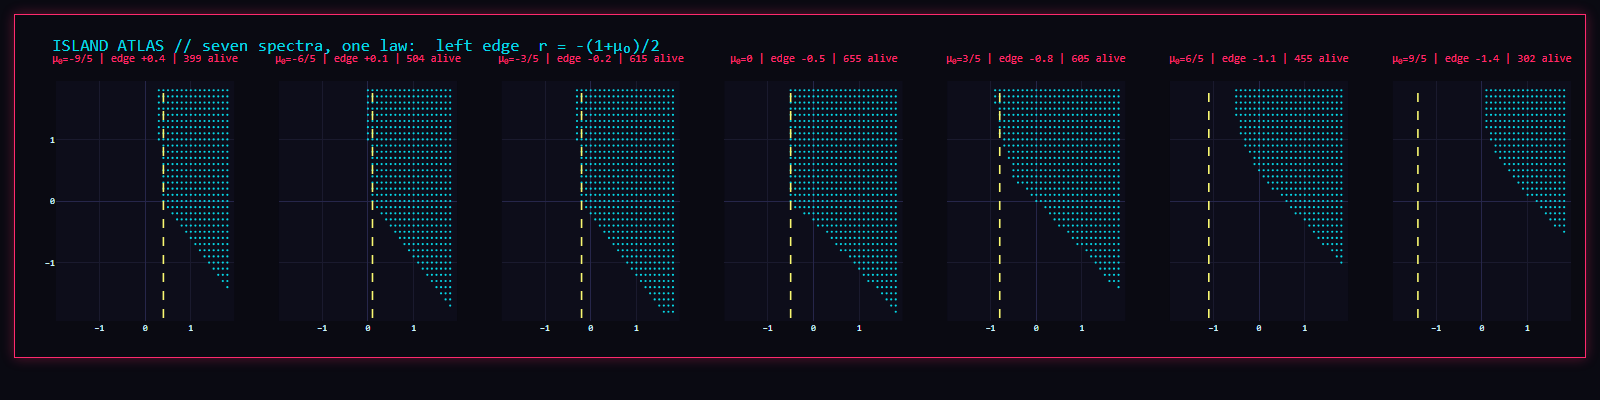
\includegraphics[width=\textwidth]{fig_atlas.png}
\caption{Positivity islands for seven mass shifts $\mu_0$ (exact rational
scans; cyan = allowed). Dashed line: the exclusion edge $r=-(1+\mu_0)/2$. For
$\mu_0\le 0$ the island reaches the line; for $\mu_0>0$ threshold constraints
cut strictly inside it.}
\label{fig:atlas}
\end{figure}

\begin{figure}[t]
\centering
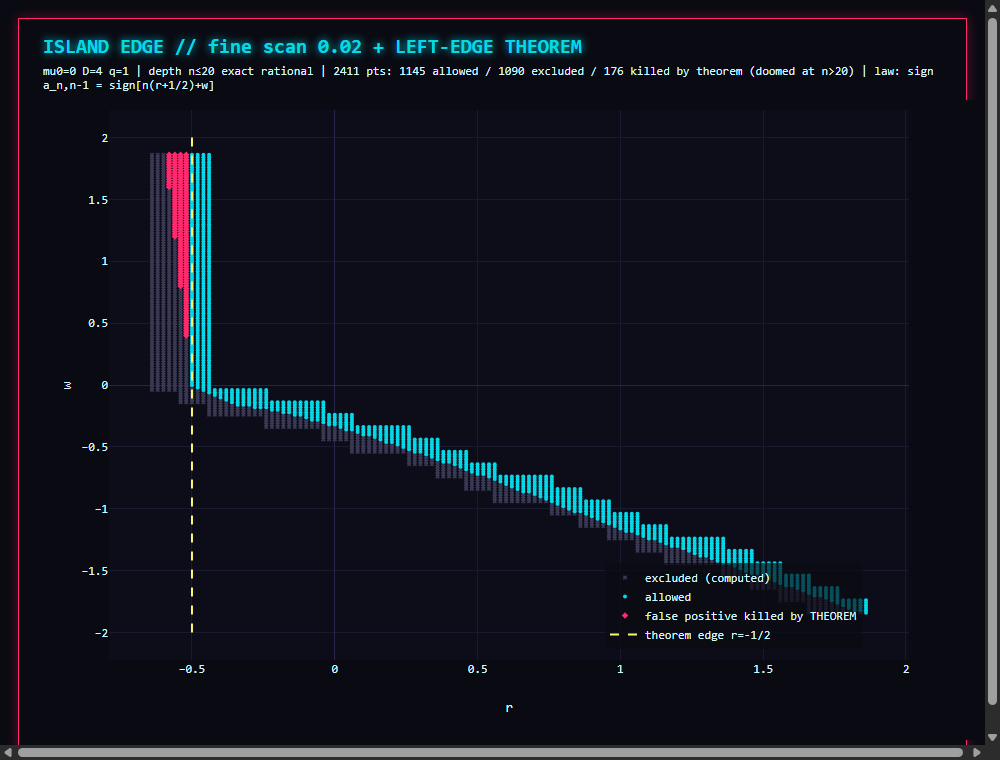
\includegraphics[width=0.9\textwidth]{fig_edge.png}
\caption{Fine boundary scan at resolution $0.02$ ($\mu_0=0$, depth $n\le 20$).
Cyan: allowed; grey: excluded by direct computation; pink diamonds: the $176$
points admitted by the finite-depth scan but excluded by the ladder law, each
with its predicted death depth; dashed line: $r=-1/2$.}
\label{fig:edge}
\end{figure}

\textbf{Threshold structure at $\mu_0>0$.} The dominant killers sit at the
first above-threshold level ($n_{\min}=2,4,6$ for $\mu_0=3/5,6/5,9/5$),
predominantly the scalar channel: as $\alpha\to 0$ the residue degenerates
toward pure $\ell=0$. The scalar curve is explicit, e.g.
$a_{2,0}(r,w,\mu_0)\propto 6\mu_0^2+6\mu_0 r+3\mu_0 w-3\mu_0
+6r^2+6rw+6r+6w+2$, factoring at $\mu_0=2/3$ as $(3r+4)(3r+3w+1)/9$.

\textbf{Dimension dependence.} With the positive factor
$\sqrt{\pi}\,\Gamma(\tfrac{D}{2}-1)/\Gamma(\tfrac{D}{2}-\tfrac12)$ removed,
$a_{1,0}\propto r+w+\tfrac12$ is $D$-independent, while
\begin{equation}
a_{2,0}\;\propto\;(1+r)(r+w)+\frac{1}{D-1},
\end{equation}
and $a_{3,0}$ carries analogous $1/(D-1)$ coefficients. The island therefore
shrinks with $D$ through a $1/(D-1)$ tightening of its scalar curves --- an
analytic account of CHR's numerical observation --- while its left edge stays
pinned at $-(1+\mu_0)/2$ in every dimension.

\textbf{Fixed-spin tails.} Localizing the projection at $x=1$ gives
$a_{n,\ell}\sim (2\ell+1)\,C(r,w)/(n\ln n)$ with $C>0$ across the domain; the
$(2\ell+1)$ scaling agrees to three digits between $\ell=0$ and $\ell=2$ in
exact numerics, with positivity checked up to $n=200$ at representative points,
while the constant converges logarithmically. This part is heuristic-plus-numeric.

\section{The $q$-clock}

For $q>1$ CHR excluded the deformation asymptotically. Using their Eq.~(16)
directly (roots $\xi(k)=[-1-r-k]_q$ are bounded by $-1/(q-1)$ while the angle
substitution grows as $[n]_q\sim q^n$), we scanned the $q$-Veneziano line
($r=w=0$) in exact arithmetic and measured the depth at which the first
negative partial wave appears:
\begin{center}
\begin{tabular}{lcccccc}
\toprule
$q-1$ & $0.001$ & $0.005$ & $0.01$ & $0.02$ & $0.05$ & $0.1$\\
$n_{\rm crit}$ & $34$ & $15$ & $11$ & $8$ & $5$ & $4$\\
\bottomrule
\end{tabular}
\end{center}
consistent with $n_{\rm crit}\simeq 1.1\,(q-1)^{-1/2}$ over two decades (the
$q=1$ control is clean to $n=25$; the killer is low spin, $\ell=0,1$, not the
ladder). The exponent follows from the logarithmic derivative (computed as an exact
finite difference at step $10^{-6}$)
$-\partial_q \log a_{n,0}\big|_{q=1}\approx 0.3\,n^2$: the relative
$q$-correction grows quadratically (the spectrum drift $[n]_q\approx
n\bigl(1+\tfrac{(n-1)(q-1)}{2}\bigr)$ accumulates), so the crossing occurs at
$(q-1)\,n^2=O(1)$. This yields a practical corollary: any depth-$N$ scan
necessarily admits $q-1\lesssim (1.1/N)^2$, quantifying the $q$-tolerance of
finite numerical bootstraps (e.g.\ $q-1<0.012$ at CHR's depth $10$).

\section{Relation to prior work}

Mansfield and Spradlin \cite{MS2024} analyzed the $w=0$ (hypergeometric)
slice of this family with double-contour methods. Their odd-$\Delta$ Regge
asymptotics carries the overall factor $(2r+m^2+1)$ --- asymptotic positivity
requiring exactly our edge line at $w=0$. The two approaches agree where they
overlap, while Theorem~\ref{thm:edge} is exact at every finite level and
covers $w\neq 0$, which their analysis does not treat. Within the $49$ works
citing CHR we found no other treatment of the $w\neq 0$ region or of the
island's infinite-depth fate.

\section{Discussion}

Within CHR's explicitly stated assumptions, the boundary of the space of
consistent Veneziano neighbors is no longer a numerical scan but a short list
of explicit algebraic conditions, with one conjectural completeness statement
that survived every falsification attempt we could construct
($11{,}994$ exact verdicts; adversarial review; thirty successful
doomed-cell predictions; eight razor zeros). The natural next steps are a
general-$k$ proof of the odd-trajectory dichotomy, a rigorous fixed-spin
asymptotic, and --- toward quantum gravity --- transplanting the
top-coefficient method to families with double zeros in their residues
(Virasoro--Shapiro-like), where CHR posed the corresponding uniqueness
question for gravitational amplitudes.

\section*{Reproducibility and AI disclosure}

All computations are exact-rational and scripted; the repository contains the
two-route evaluator, all maps and scans, the razor tests, the independent
reviewer's attack script, and the append-only research log. This research was
conducted by the author working with an AI research assistant (Claude,
Anthropic); every scientific claim above was verified by deterministic code
whose outputs are published, and the assistant's derivations passed an
independent adversarial review recorded in the repository.

\begin{thebibliography}{9}
\bibitem{CHR2024} C.~Cheung, A.~Hillman and G.~N.~Remmen,
``Bootstrap Principle for the Spectrum and Scattering of Strings,''
Phys.\ Rev.\ Lett.\ 133, 251601 (2024), arXiv:2406.02665.
\bibitem{MS2024} G.~Mansfield and M.~Spradlin,
``On Unitarity of the Hypergeometric Amplitude,''
arXiv:2409.09561.
\end{thebibliography}

\end{document}
